\documentclass[twocolumn,10pt]{article}
%\documentclass[conference,10pt]{IEEEtran}
\usepackage{epsfig,endnotes}
\usepackage{mathptmx}
\usepackage{epsfig,color}
\usepackage{cite,url}
\usepackage{amsmath}
%\usepackage{usenix}
\usepackage{algorithm}
\usepackage[noend]{myalgorithmic}
\usepackage{times}
\usepackage{alltt}
\usepackage{xspace}
\usepackage{amsthm}

\usepackage[margin=1in]{geometry}
\usepackage[medium,compact]{titlesec}

\date{}

%\usepackage[bigsym]{amsmath}
%\pagestyle{empty}
\begin{document}

\newtheorem{theorem}{Theorem}
\newtheorem{lemma}{Lemma}
\newtheorem{definition}{Definition}

\newcommand{\bihq}{BI-HQ\xspace}
\newcommand{\msg}[1]{\ensuremath{\textsc{#1}}}
\newcommand{\note}[1]{[\textcolor{red}{\textit{#1}}]}
\newcommand{\stitle}[1]{\vspace{2pt}{\bf #1:}}
\newcommand{\priority}[1]{[\textcolor{blue}{\textbf{#1}}]}

%%%%%%%%%%%%%%%%%%%%%%%%%%%%%%%%%%%%
%%%%%%%%%%%%%%%%%%%%%%%%%%%%%%%%%%%%
%% Set to #1 for technical report
%% Set to #2 for submission
%%%%%%%%%%%%%%%%%%%%%%%%%%%%%%%%%%%%
%%%%%%%%%%%%%%%%%%%%%%%%%%%%%%%%%%%%
\newcommand{\reportsubmission}[2]{#2}
%%%%%%%%%%%%%%%%%%%%%%%%%%%%%%%%%%%%
%%%%%%%%%%%%%%%%%%%%%%%%%%%%%%%%%%%%



%%%%%%%%%%%%%%%%%% Structure of the HotOS paper %%%%%%%%%%%%%%
%% Motivation for weakly consistent BFT protocol %%%%%%%%%
%% Target applications where it could be used %%%%
%% System protocol and architecture
%% Preliminary results

%\title{Bounded-inconsistent BFT Protocols: Trading consistency for throughput}
\title{Safe Hints in
Byzantine Fault-Tolerant Distributed Services}
\author{Atul Singh$^{\dag}$,
Petros Maniatis$^{\ddag}$, 
Peter Druschel$^{\phi}$,
Timothy Roscoe$^{\star}$
\\
Rice University$^{\dag}$, Intel Research Berkeley$^{\ddag}$, MPI for
Software Systems$^{\phi}$, ETH Z\"urich$^{\star}$}

 % make the bibliography compact
 \let\oldthebibliography=\thebibliography
 \let\endoldthebibliography=\endthebibliography
 \renewenvironment{thebibliography}[1]{%
     \begin{oldthebibliography}{#1}%
     \setlength{\parskip}{0ex}%
     \setlength{\itemsep}{0ex}%
 }%
 {%
     \end{oldthebibliography}%
 }



\maketitle
\begin{abstract}
We identify and articulate a design pattern in Byzantine state machine
replication protocols, which we call \emph{safe hints}. Safe hints
allow an untrusted component to produce easily verifiable hints, which
improve performance in the common case. We first identify uses of safe
hints in existing protocols. Then, we propose two novel protocol
optimizations based on safe hints and present a preliminary analysis
to show their effectiveness.
\end{abstract}

\section{Introduction}
\label{sec:introduction}

Protocols for Byzantine-fault tolerant replicated state machines (BFT
RSM) have received a lot of attention, and several practical
implementations have been proposed~\cite{Castro1999, fault-scalable-sosp-05,
hq-replication-osdi-06}. In this paper, we observe
and articulate a common design pattern in BFT RSMs, which we call
\emph{safe hints}. In a typical use of this pattern, a replicated state 
machine is bracketed with an \emph{untrusted hint generator} (UHG) and
a \emph{safety validator} (SV).  The key idea is to let the hint
generator produce hints that can be subsequently verified by the
safety validator.  The hints are designed to improve performance in the
common case where the hint generator is correct and the hint turns out
to be safe and effective.  Examples of hints are the batching and
reordering of requests, or the speculative completion of requests by a
subset of the replicas.

The safe hints pattern can be recognized in existing BFT protocols.  For
example, the primary replica in the PBFT protocol~\cite{Castro1999}
proposes an ordering of requests, which other replicas verify for
correctness before executing. Moreover, safe hints are closely related
to speculative techniques used in other types of systems, including
distributed systems~\cite{Speculator-sosp-05} and hardware branch
prediction~\cite{Hardware-compiler-branch}. In this paper, we contend
that the safe hints pattern, once recognized in the context of BFT,
enables new, safe optimizations of BFT protocols. Moreover, we believe
that safe hints simplify reasoning about BFT protocols.

We present two novel optimizations of BFT RSMs based on safe hints.
First, we describe \emph{HQ++}, a novel variant of HQ~\cite{hq-replication-osdi-06}. HQ++
realizes the advantages of HQ even under high-concurrency workloads,
thus removing the principal limitation of HQ. HQ++ (described in
Section~\ref{sec:hq++}) adds to HQ an untrusted hint generator that
pre-serializes requests. The untrusted hint generator can also implement 
batching (like PBFT and unlike HQ) and amortize the overhead over several requests, 
improving HQ++'s performance further.

% I thought batching needed more bragging since it is a great weapon for PBFT.
% HQ can not do it nor other quorum protocols. So, I tried to add more text about it
% - Atul.

Second, we show how safe hints can be used to construct BFT RSMs that
trade consistency for throughput and request latency. We describe
\emph{BI-HQ}, a bounded-inconsistency protocol based on HQ. BI-HQ
(described in Section~\ref{sec:bihq}) uses a hint generator that
allows replicas to unilaterally respond to requests, whenever the
replica can ensure, based on its local state, that a tentative response will
not violate a given inconsistency bound.  Figure~\ref{fig:Examples}
illustrates schematically safe hints for existing systems, as well as
for the contributions of this paper.

\begin{figure*}
\centering
%\includegraphics[width=3in]{Examples.eps}
\includegraphics{Examples.eps}
\caption{Examples of Safe hints.
}
\label{fig:Examples} 
\end{figure*}



The two novel uses of safe hints we present here are surprisingly
simple (in retrospect), yet powerful.  We show preliminary analytical
evidence justifying our optimism in Section~\ref{sec:analysis}.



\if 0
Protocols for Byzantine-fault tolerant replicated state machines (BFT
RSM) have received a lot of attention. This attention is well deserved
as these protocols promise to provide a powerful tool for the
construction of robust services. With BFT RSMs, programmers can write
sequential, fault-oblivious code that implements a server state
machine. The protocol then ensures that the replicated server state
machine executes requests sequentially and atomically
(\emph{linearizability}), that it makes progress despite transient
network faults (\emph{liveness}), and that it can mask a bounded number
of arbitrary replica failures.

There are two general types of BFT RSM protocols. The Practical
Byzantine Fault Tolerant (PBFT) protocol~\cite{Castro1999} and its
derivatives use 3-round Byzantine consensus over $3f+1$ replicas to
ensure that all clients' requests are executed in a consistent order
in the face of up to $f$ replica faults.
Q/U~\cite{fault-scalable-sosp-05}, on the other hand, is an example of
a single-round quorum-based protocol that tolerates up to $f$ faulty
replicas within a set of $5f+1$ replicas. Replicas optimistically
execute requests locally without explicitly agreeing on a common
order. When an ordering conflict is detected among replicas, client
requests need to be aborted and retried to resolve the conflict.

Consensus- and quorum-based protocols differ in the number of replicas
required to tolerate $f$ faulty replicas. Moreover, variants of each
type of protocol differ in their performance characteristics under
different workload conditions. Common to all BFT RSM protocols,
however, are limitations in terms of performance and scalability.
PBFT requires a quadratic number of messages in the number of replicas
and three rounds of message exchanges. This limits scalability to
large replica groups (i.e., large $f$), causes low throughput in
bandwidth-constrained environments, and causes high request latency
when the network delay among replicas is high.  Q/U requires a
significantly lower number of messages and fewer rounds, but can be
mired by livelock under high-concurrency workloads, where multiple
clients issue requests to the RSM concurrently.

To deal with these performance limitations, the HQ protocol by Cowling
et al.~\cite{hq-replication-osdi-06} combines the quorum and consensus
approaches in an ingenious way.  HQ is a quorum protocol in the
absence of conflicting write requests (a common case). Upon detecting
concurrent requests, it resorts to Byzantine consensus for efficient
conflict resolution.  The relatively expensive consensus is only used
to resolve concurrency conflicts, which would require exponential
back-off in a pure quorum system such as Q/U.  As a result, HQ
improves significantly upon PBFT in low-concurrency
settings,
while resolving concurrency conflicts at a lower expected
latency than Q/U.

The ``magic'' in HQ's conflict resolution technique relies on utilizing an untrusted, centralized
agent (called a \emph{proxy server} in that work). The proxy collects
conflicting requests opportunistically, combines them into a conflict
resolution batch, and submits them to the PBFT module for
linearization. Once the order of conflicting requests has been agreed
upon, the replicas validate the conflict batch: they check whether a
conflict resolution was really needed, and whether all conflicting
requests are valid.  Then, they either execute the valid batch of
conflicting requests in a consistent order, or otherwise reject the
batch, replace the faulty proxy server that produced the batch via a
PBFT view change, and try again.

In this paper, we observe that HQ's approach can be viewed as an
instance of a protocol structuring pattern we call a \emph{safe hint}.
Safe hints typically look like a bracketing of a service (e.g., PBFT
in HQ's case) between an \emph{untrusted hint module} (UHM) and a
\emph{safety validator module} (SVM). In the case of HQ's conflict
resolution subprotocol, the proxy server acts as the UHM and the
execution quorum acts as the SVM, ensuring that only valid conflict
resolution batches are handled. The key idea behind safe hints is to
let untrusted replicas produce easily verifiable hints, which will
improve performance in the common case. This case occurs whenever the
hint generator is correct and the hint turns out to be useful.
%Examples
%of such hints are the batching, reordering or speculative execution of
%requests.

The safe hints pattern is not new. It can be seen in HQ and in other
BFT RSM protocols. For example, the primary replica in the PBFT
protocol optimistically proposes an ordering of requests, which other
replicas verify for correctness before executing. However, we show
that the safe hint pattern, once recognized as a general technique,
enables many additional safe optimizations of BFT protocols.
Moreover, we observe that the safe hint pattern enables the
application of hint-based techniques in BFT systems, even though these
techniques were originally developed for systems with crash failures.  For
instance, we show that safe hints allow us to apply existing
techniques to BFT RSM systems to relax consistency in exchange for
improved performance~\cite{Satyanarayanan2002,Terry1995,Yu2002}.  We
present two instantiations of the safe hints pattern for both
performance optimizations and functionality extensions to support this
claim.

First, we build \emph{HQ++}, an HQ variant that, under fault-free executions,
avoids conflict resolution and hence consensus
\emph{entirely} by placing a 
pre-serializer UHM before HQ (Section~\ref{sec:hq++}).  Even if the pre-serializer
is faulty, HQ++ can easily detect and replace it with another pre-serializer and
make progress. Second, we show how safe hints
can help relax the consistency of BFT RSMs to improve throughput and
client latency. We build \emph{BI-HQ}, a bounded-inconsistency
protocol reminiscent of TACT~\cite{Yu2002}, which is based on HQ (it
can also work with Q/U or PBFT). BI-HQ places a UHM at each replica,
which locally responds to requests that appear not to violate an
inconsistency bound. Once the bound is reached, the requests are
submitted to the HQ. BI-HQ validates the safety of the consistency protocol
by placing an SVM after HQ to ensure that only those linearized requests
commit which do not violate the inconsistency bound.

%of the RSM and the
%inconsistency bound by placing an SVM after HQ to execute linearized
%requests.
%Third, we further improve BI-HQ's performance by using an untrusted
%batch consolidator before HQ, reducing the number of RSM invocations
%from $(2f+1)$ to one per bounded-inconsistency synchronization
%(Section~\ref{sec:bihq}).

The two novel examples of safe hints we present here are (in
retrospect) surprisingly simple, yet surprisingly powerful. HQ++ need
never resolve conflicts, as long as pre-serializer is non-faulty. HQ++ can
amortize the protocol overhead cost over several requests via batching while
HQ can not.
BI-HQ opens up a new avenue for exploiting different types of weak consistency
in Byzantine environments.  We show preliminary analytical evidence
justifying our optimism (Section~\ref{sec:analysis}). \note{Next lines are slightly abstract.}
We also sketch our future research
agenda in this space, where we intend to cast other performance or
functionality improvements for BFT systems as safe hints. Such
improvements can be used to safely generalize or customize a protocol ensemble
to its target environment.
\fi





























\section{HQ++: Pre-serialization for HQ}
\label{sec:hq++}

Our first novel application of safe hints allows us to build an
extension of the HQ protocol that extends HQ's benefits over
PBFT under all workload conditions.

\subsection{Background: HQ}

HQ~\cite{hq-replication-osdi-06} combines quorum- and consensus-based
BFT approaches.  HQ acts like a quorum protocol in the common case
where clients are non-faulty and there are no concurrent write
requests.  When faults or concurrent writes occur, HQ resorts to PBFT
to manage conflict resolution.  Like PBFT and other BFT replicated state
machines, HQ guarantees the \emph{linearizability} property, according
to which completed client requests
appear in a unique, totally ordered,  serial  
schedule.
%HQ requires $3f+1$ replicas to tolerate $f$ faults among replicas and
%any number of faulty clients. 

Common case read operations complete in a single round-trip. Common
case writes require two round-trips. A client first issues a write
request to all replicas and expects from each replica a \emph{grant}
to execute its request with a particular sequence number.  Once the
client has collected a quorum of $2f+1$ such matching grants,
forming a \emph{write certificate}, it submits them to the replicas. A
replica that receives a correct write certificate for a request
executes it using its local state and sends the result to the client.

Write contention is detected by a client when it receives a quorum of
grants for the same sequence number but different requests.  In this
case, the client submits this set of responses, called a
\emph{conflict certificate}, to all replicas, in a \msg{Resolve} message.  Then, a replica initiates 
conflict resolution by sending to the proxy server (PBFT's primary) a
$\textsc{Start}$ message containing the conflict certificate provided
by a client.  When the proxy server collects a quorum of $2f+1$ such
messages, it submits a PBFT conflict resolution request containing all
conflicting client requests to PBFT for linearization.  Once the
conflict resolution is committed by PBFT, replicas execute the client
requests contained in the quorum of $\textsc{Start}$ messages in a
consistent order.


\subsection{HQ++ Design}

In the absence of significant write concurrency, HQ is more efficient
than PBFT, at the expense of increased overhead during high
concurrency.  HQ++ is able to deliver the same performance
irrespective of the level of concurrency.

In HQ++, an untrusted hint generator serializes client
requests before submitting them to HQ. As a result, concurrency
remains hidden from HQ.  In a fault free environment, HQ++ need not
perform any conflict resolution at all.  The same safety and liveness
guarantees offered by HQ are offered by HQ++.

\stitle{Clients} To clients, HQ++ appears identical to HQ.

\stitle{Hint generator} One of the replicas takes on the role of the
\emph{hint generator}: at any time, the hint generator is the $i$-th
replica, $i \equiv s \mod N$, where $s$ is the current sequence
number of the PBFT protocol for conflict resolution, and $N=3f+1$ is
the number of replicas\footnote{In the general case, a hint generator
might also be chosen from the client population, or be an entirely
separate node.}.

The hint generator buffers client requests and submits them to the %batches to the
HQ replicas, serially, as a regular HQ client.  Once it has received a
quorum of $2f+1$ acknowledgments from distinct HQ replicas (a signed hash
of its request), it can submit the next serialized client request. % batch.

%%% Removed the batches from discussion here. We discuss batching later
%%% as an optimization later. - Atul.

\stitle{Replicas} HQ++ replicas behave identically to HQ replicas with one
exception: though they see regular clients' requests, they do not
process them immediately. Instead, they associate a timer with each.
When the same request is received from the hint generator, the replica
cancels the timer, sends a grant to the client and an
acknowledgment to the hint generator.  If the timer for a client's
request expires before that request is received from the hint
generator, the replica initiates a hint generator change (see below).
A client request that arrives at a replica after it was received from
the hint generator is ignored.



\stitle{Faulty hint generators} A hint generator, like any other
replica, may be faulty. To other HQ replicas, it appears as a faulty
client that might submit different requests to different replicas.  To
clients, a faulty hint generator might cause delay (by suppressing a
client request) or a write conflict. 

\stitle{Faulty clients} Since HQ++ relies on clients to perform the
second phase of the write protocol, a faulty client may delay writes. In HQ, if replicas receive a
new write request for an object for which there is a pending write,
they send a refusal response to the request, prompting the new client
to complete the previous request.  We use the same approach to handle
faulty clients in HQ++.  Note that unlike in HQ, faulty clients cannot
force HQ++ into conflict resolution by submitting different requests
with the same request identifier (RID) to different replicas (RID is assigned 
by the client to every request it sends). This is because in HQ++,
requests are not given a grant at the replicas until they are serialized.
Once serialized, a request that encounters at a replica a disparate
signed request by the same client,  invalidates the timer of that
request. 

%y cannot submit
%different requests to different replicas without being detected as
%faulty when the version sent by the hint generator is received.
%\note{please check above for accuracy. -PD}

\stitle{Hint generator change} Replicas handle hint generator changes in
the same way HQ handles conflict resolution. A replica sends a
\textsc{Start} message that may contain a conflict certificate (if the
faulty hint generator submitted conflicting writes to different
replicas) or not (if the hint generator suppressed a client request
causing timers to expire).  Conflict resolution eventually results in
a PBFT invocation, which increments the PBFT sequence number and
resolves any conflicting writes.  Note that incrementing the PBFT
sequence number changes the hint generator. The cost of
changing the hint generator is similar to the cost of resolving
conflicts in HQ.

\stitle{Informal Correctness} Our modifications of HQ do not affect safety
because HQ can tolerate an arbitrary number of faulty clients. Since a
faulty hint generator at worst appears as a faulty client to HQ
replicas, safety is
preserved.  However, a faulty hint generator may affect liveness,
since it may attempt to suppress or unduly delay a correct client's
request. However, as described above, this results in an eventual hint
generator change. Therefore, progress is ensured as long as clients
retransmit their requests until they succeed.

Since hint generators need not be trusted, their task fits the UHG
role of the safe hint pattern. The conflict resolution protocol and
the request timers at the replicas fit the SV role of the pattern.

\subsection{Batching in HQ++}

The hint generator can combine multiple client
requests into a single batch. Replicas, upon receiving such a batch,
create a cumulative grant for the entire batch and send it to a client
chosen deterministically from the batch (e.g., the owner of the first
request in the batch).  A non-faulty client creates a write certificate
for the batch and sends it again to the replicas in phase 2.  Replicas
then send a reply message for every request in the batch to the client
who issued that request.  Note that replicas create a single grant for
the entire batch. As a result, they save processing (they
compute a single
authenticator as opposed to one per included request) and bandwidth
(they transmit a single grant as opposed to one per included request)
proportional to the batch size.

\stitle{Correctness} A faulty client may fail to submit the write
certificate for the whole batch. This is equivalent to a regular
client who fails to perform the second phase of the protocol, which is
already handled by HQ. If a faulty hint generator attempts to submit
batches that omit some requests, a similar timeout occurs as with HQ++
without batching.  Finally, if a hint generator submits different
batches to different replicas, HQ reacts as if it had received
conflicting requests from a faulty client, which is resolved after the
hint generator has been changed.


\subsection{Switching between HQ and HQ++}

Under very low contention, HQ++ incurs slightly more bandwidth and
latency overhead than HQ, since the hint generator retransmits client
requests to HQ replicas.  This suggests that one should use HQ under
low contention but safely switch to HQ++ if contention increases.  We
briefly describe how to implement such a protocol switch as a safe
hint.

The switching mechanism is analogous to conflict resolution based on
PBFT.  While in HQ mode, when a replica notices it sees many
\msg{Resolve} requests compared to few uncontested request  executions
in the same time window, it sends to the PBFT primary (the proxy server) a
\msg{Start} message containing a \msg{HqToHq++} payload.  When the proxy
server collects a quorum of $2f+1$ such messages, it bundles them
together into a switch certificate, which it submits to PBFT for
linearization.  When executed in PBFT, the switch certificate, if valid, causes the executing quorum
of replicas to switch to HQ++.  Switching from HQ++ to HQ happens
similarly, and is triggered when a replica notices that its buffer of pending client
requests, waiting for pre-serialization by the hint generator, is mostly
empty for a sustained period of time.  Hysteresis in the switching
triggers (on non-faulty replicas) is used to avoid oscillations.
Note that faulty replicas cannot cause oscillations alone, since a
quorum of $2f+1$ triggers are required to switch.

Finally, non-faulty replicas that did not participate in the PBFT quorum
that committed the switch find out about the switch during regular PBFT
state transfers (aimed at bringing lagging replicas up to speed with the
committed history of the system).

































\section{Bounded Inconsistency BFT}
\label{sec:bihq}

Relaxing consistency is a widely used technique to improve the
performance of replicated
systems~\cite{Satyanarayanan2002,Terry1995,Yu2002}.  Applications that
can tolerate bounded inconsistency may trade consistency for increased
throughput and reduced delay. Examples of such applications in the BFT
domain include, for instance, quota enforcement for fair sharing P2P
applications.  In this section, we present a bounded-inconsistency BFT
protocol that uses the safe hints pattern.

\subsection{Background: TACT}
We focus on bounded-inconsistency systems as introduced by
TACT\cite{Yu2002}.  TACT provides a framework for applications to
specify their consistency requirements for accesses in a replicated
system.  A replica may tentatively reply to a client request
immediately, before that request is committed to all replicas of the
system's state. Therefore it may produce an inconsistent result.
Applications specify an acceptable consistency bound using different
metrics. For instance, a numerical error metric is defined to be the
\emph{weight} of updates that the inconsistent, tentative
result to an operation could miss that 
it would have otherwise seen in a strictly consistent
(linearized) execution, for some
application-specific weight function (defined as a
\emph{conit} function $F$).
Consider an airline reservation system in which
bumped customers of overbooked flights receive a compensation.
A weight
function for every reservation request would be the compensation that
the airline would owe if that reservation could not be honored due to
overbooking.

In TACT, inconsistency is \emph{bounded}, since replicas give a
tentative reply to a client's request only if that reply's
inconsistency is guaranteed to be within a given bound.  In the
airline example, the bound could be the airline's total budget for
compensations due bumped customers.

In crash-fault environments, TACT provides bounded inconsistency with regards to
numerical error by allowing each individual replica to locally process clients' requests, as
long as the total weight of those tentative requests does not surpass a local bound
$\beta$. When a new request arrives that could cause that bound to be
violated, the replica propagates its updates to all other replicas
synchronously before tentatively replying to the newly arrived
request.  The global numerical error bound $\alpha$ is set by the
system administrator; the local-replica bound $\beta$ is derived from
$\alpha$ and the number of replicas in the system. In TACT, $\beta=\alpha/(N-1)$, where
$N$ is the number of replicas.







\subsection{Design}
BI-HQ uses a consistency protocol similar to TACT, and HQ as the
synchronization back-end.  BI-HQ replicas are clients of HQ, proxying
end users' requests to HQ. For simplicity, we only consider numerical error in
this paper.

\stitle{Clients}
A client sends a request to all BI-HQ replicas and waits for $2f+1$
matching replies before considering the request $\emph{completed}$.
The client maintains a timer for each pending request. If the timer
expires, the client retransmits the request.

As with TACT, \bihq guarantees that the result of a completed request
can at most miss updates of weight $\alpha$ that it would have otherwise
seen in the system's linearized request ordering.
%lies within an application-specified numerical error bound $\alpha$ from
%the result that request will eventually produce when executed in the
%system's linearized request ordering.  
\bihq is also live: it
ensures that a non-faulty client eventually gets its pending
requests completed.

%Submitted but not completed
%requests \emph{may} eventually be committed, but no guarantee is given
%on their reply value. \note{I don't get the last sentence. -PD}
For presentational purposes, we logically separate the functionality
of BI-HQ replicas into two parts: BI and HQ replicas. In practice, the
two parts are implemented by the same physical machine.

\stitle{BI Replicas} Each BI replica -- acting as the UHG 
in the safe hints pattern -- is an HQ client.
% as well as an HQ replica.
%client and server state. 
In addition, a BI replica maintains a list $T$ of
tentative requests that it has received and tentatively responded to
since the last synchronization, the last synchronized service state 
and the largest request timestamp it has processed for every client.
The BI replicas interact with clients.

\stitle{HQ Replicas} These replicas implement the HQ protocol. 
These replicas do not interact with clients.

%Each BI-HQ replica -- acting as the UHG
%in the safe hints pattern -- is an HQ client maintaining all HQ
% client state. In addition, a BI-HQ replica maintains a list $T$ of
%tentative requests that it has received and tentatively responded to
%since the last synchronization, 
%the latest sequence number for the
%synchronized service state (e.g., the object version ID for HQ), and
% the largest request timestamp it has processed for every client.

\stitle{Client request handling} When a BI replica receives from client $c$ a new request 
(with a timestamp
larger than the largest known timestamp by client $c$)\footnote{A
request with an earlier timestamp than the latest seen for that client
is treated as a retransmission and may be handled using a local
cache. We omit the (straightforward) details here for brevity.}, it
ensures that this new request, if tentatively executed, would
not cause it to violate its local inconsistency bound $\beta$.
%, as described below in the \emph{error-bounding} discussion. 
 Then, it appends the request to its buffer $T$ and produces a
 tentative reply based on its local state, to which it applies all
 tentative requests in $T$ sent by client $c$.  It returns to client
 $c$ the computed result $r$ in a reply message.

\iffalse
Restricting tentative requests to receiving replies based only
on the same client's tentative requests s ensures that the client
receives ``read your writes'' session guarantees on its own tentative
requests between checkpoints.
\fi


\stitle{Error bounding} A BI replica checks if the inclusion of the new client request
into the tentative requests $T$ would cause neither the total
positive weight nor the total negative weight of tentative requests to
exceed a threshold $\beta$, then error bounding is complete and it
can continue handling the request as described above.

Otherwise, the BI replica invokes a synchronization
round, by bundling its tentative request in $T$ (excluding the newly
arrived request) into a single HQ request (called a \emph{BI batch}) and 
invoking the HQ protocol
as if it were a regular HQ client.  The replica handles the offending 
client request  and any future
requests only after the synchronization round is complete.
Once complete, the BI replica flushes
$T$ and applies the requests contained in the synchronization response to its local state.
A synchronization response contains a unique BI batch from a quorum of $2f+1$ replicas. BI
replicas associate a timer with the synchronization request. If the timer expires before
the synchronization round is complete, the BI replica multicasts the tentative list $T$ of
requests. 
%its bundled synchronization request has been
%completed.
%, as per the definition of completed requests in HQ.






\stitle{Synchronization round} The last piece of the puzzle involves the SV
component of safe hints: the verification and execution of the BI batch
stream, as linearized by HQ.
When a BI batch
is linearized by HQ replicas and
reaches the execution phase, the HQ replica first verifies that the
tentative requests in
the BI batch
do not violate the local error bound $\beta$. If the test succeeds, the
HQ replica buffers the
BI batch and sends an HQ reply to the BI replica that submitted the BI batch. Note that
this reply does not yet conclude the synchronization and the BI replica
is still blocked.
Once HQ replicas have linearized a quorum of $2f+1$ BI batches by
distinct BI replicas, they send all
these batches to the BI replicas of each included BI batch.

As explained before, once a BI replica receives a quorum of $2f+1$
linearized BI batches, each
from a different BI replica, it executes
and commits the requests contained in these batches in a deterministic
order to its
local state.
This marks the completion of the synchronization
round and BI replica can process further requests.




\stitle{Informal Correctness} For safety, first we need to ensure that $2f+1$
valid BI batches contain requests of at most $\alpha$ weight. Second, we 
need to show that every completed request appears in at least one of the $2f+1$
valid batches. We ensure the first property by observing
that BI replicas request synchronization
once they have collected requests of weight $\beta$ in a BI batch.  Replicas
only commit requests in the local state when BI batches from $2f+1$ unique replicas 
have been committed by HQ. Let these replicas form a quorum $Q$.  Setting
$\beta=\alpha/(3f+1)$, we are ensured that the weight of requests
contained in these BI batches is bounded by $\alpha$. 
By definition of a
completed request, at least a quorum of $2f+1$ replicas responded,
call it $P$. By the quorum intersection property, at least one
non-faulty replica is common to $P$ and $Q$ and the completed request
appears in that replica's BI batch. Hence, the second claim holds. Our safety
guarantee, i.e., the numerical error seen by a completed request is bounded by $\alpha$, 
follows from these two claims.
% Hence, our safety guarantee of bounding
%the numerical error of a completed request by $\alpha$ follows.
For liveness, we have to ensure that BI replicas do not wait indefinitely
to complete the synchronization round. 
BI replicas associate a timer with the synchronization requests. If the timer expires
before the synchronization round completes, the BI replica multicasts its list $T$ of 
requests to other replicas. This ensures that other non-faulty replicas would also initiate
the synchronization and complete the synchronization round.

\stitle{Pre-batching} BI-HQ only executes and commits requests in
the local state when $2f+1$ BI batches 
have been committed by HQ. A natural performance optimization, which
we can implement as a separate safe hint, is to pre-integrate the
$2f+1$ BI batches of tentative updates in a single batch and then submit
that batch to HQ for validation and execution.  Viewed another way,
this uses HQ++ instead of HQ in BI-HQ. Whereas the original BI-HQ executed HQ $2f+1$ times to
perform a single synchronization, the BI-HQ++ executes HQ++
\emph{only once} per synchronization, reducing overheads
significantly.  We omit the details  for lack of
space~\cite{hq++:website}.


\if 0
%% Removed this detailed description for space.

\section{Pre-integration to Improve BI-HQ Performance}
\label{sec:bihq++}

BI-HQ only commits requests when $2f+1$ batches have been committed by
HQ. A natural performance optimization, which we can implement as a
separate safe hint, is to pre-integrate the $2f+1$ batches of tentative
updates in a single batch and then submit that to HQ for validation and
execution.  Viewed another way, one can combine BI-HQ with HQ++ as the
underlying BFT RSM protocol.

As with HQ++, in BI-HQ++ the pre-integrator is the only HQ client
allowed to submit requests to HQ.  Once it receives a single set of
updates from a replica, it pulls existing updates from other replicas
until it has collected $2f+1$ sets, which it validates to ensure they do
not violate the local $\beta$ error, and bundles them into a single batch
request to HQ.

The SVM at HQ's execution phase now checks that the batch about to be
committed contains $2f+1$ tentative update sets from distinct replicas
that meet the local error bound, and rejects the bundle otherwise,
initiating a pre-integrator change similar to hint generator changes for
HQ++.  If correct, tentative updates are executed in a deterministic
total order and replies are issued to individual replicas to unblock
them.

Whereas the original BI-HQ executed HQ $2f+1$ times to perform a single
synchronization, the BI-HQ++ executes HQ once per synchronization,
reducing overheads significantly.

\fi


\section{Other safe hints}

\subsection{Speculative execution}
Goal is to reduce the response latency. Each replica,
upon receiving the request, sends the grant and piggybacks a tentative response. If a
client receives a quorum of matching grants as well as matching responses, then it
may accept that response as the early, tentative response. Note that under no
contention, this tentative response will be the final, committed response. As long as the
pre-serializer replica is non-faulty, there will be no contention and hence the 
tentative response would be a committed response. The benefit is that the response latency
drops to one RTT to a quorum of replicas.


Clients still
need to participate in the write back, and replicas still need to participate in the
second phase. 


\subsection{Divide and conquer}

Goal is to reduce the protocol overhead at high $f$. We partition
the replicas into two disjoint groups of half the sizee. Each replica still maintains the 
full system
state and executes every operation. However, only a group is responsible for the
protocol execution of requests updating or reading half of the system state, which 
we assume is composed of multiple objects (neglect transactions for now). 
Assume the system size is N and it can tolerate upto 1/3rd faults, F
(N $\ge$ 3F+1). By partitioning, we have 2 groups of size N/2. First, let us describe how the
system works. 



\paragraph{Insight} PBFT protocol can be configured for different guarantees between safety
and liveness. For both safety and liveness, we know that N $\ge$ 3F+1. But we can tolerate
more faults by trading off  liveness. For example, we can tolerate
upto 2/3rd faults and still provide safety but liveness is lost as soon as more than 1/6th 
of the replicas fail. This means that we can optimistically partition
the replicas into two groups and make each group ensure safety (at most
2/3-rd of the replicas can fail in any group of half the system size in this setting when system as a whole
has F faults) but trade liveness. When
we suspect that liveness is lost (timeouts), we fall back to the PBFT of the whole group and
that is guranteed to be safe and live. 

\paragraph{Assumptions} \note{Use of asymmetric crypto -- check this}. Each request identifies which group will
process it.  N is the system size and $F$ is the maximum number of faults that can occur
simultaneously in the system. G is the group size and $g_l$ represents the maximum number of faults
that does not affect liveness while $g_s$ represents the maximum number of faults that does
not affect safety. Note that $g_l=G/6=N/12=3F/12=F/4$ and $g_s = 2G/3=F$. So, safety is guaranteed
even when all faults occur in the same group. However, it is possible that both groups are not live.
Quorums are of size $Q_G=5/6.|G|$, where $|G|$ is the group size

\paragraph{Client access protocol} A client submits the requests to the whole system and considers
a request completed as soon as it receives $F+1$ matching responses. A client is not aware of the fact
that the system implements divide and conquer safe hints.


\paragraph{Replica Protocol: Intra-group} Primary of the group responsible for handling a request 
will propose an ordering (using Pre-Prepare message) to the requests using the PBFT protocol, with $Q_G$ as the quorums. Once a non-faulty replica has received a quorum ($Q_G$) of matching Prepare messages, then it participates in the commit phase
by sending a COMMIT message to the other replicas of its own group. Once a quorum $Q_G$ has sent a COMMIT,
a replica enters the execute phase. In this phase, the replica notifies the other group of the request that committed. 
It then waits for an ACK from (G/2+1) members of the other group and 
participates in the Inter-group protocol to notify the other group. Once a non-faulty replica receives an
ACK from (G/2+1) members of the other group, it commits the request and sends the response to the client. 


\paragraph{Replica protocol: Inter-group} Inter-group protocol is necessary to ensure that when one or both
groups loose liveness, then the whole system is able to make progress by identifying the requests that committed
in each group. Just like the original view change protocol, as long as each committed request is present in at least
$2F+1$ replicas, we are guaranteed to collect such committed requests. Now, let us describe in detail how inter-group protocol works.
Suppose replicas from group G1 need to commit requests. Each replica in G1 sends a COMMIT message to every
replica in the group G2. Replicas in G2 do not respond immediately, in fact, they wait to see a quorum $Q_G$ of matching
COMMIT messages before they send the ACK. Replicas in G2 store such COMMIT messages. 
Replicas in G1 wait for $k$ such ACK messages, where $k+5/12.N \ge (2F+1)$, i.e., a total of $(2F+1)$ replicas should see a 
given COMMIT message. This gives $k\ge\lceil G/2 \rceil+1$.


\paragraph{Liveness recovery phase} Each replica starts a timer when it receives a message. If the timer expires before the
request is executed, then it needs to take a corrective action. When a
non-faulty replica suspects that liveness is lost (timers expire), it broadcast a NEED-N-PBFT(v+1), where v is the current
view for the N-PBFT protocol. Primary of the N-PBFT
protocol waits to hear matching such messages from at least (F+1) replicas before it initiates the liveness recovery phase. Essentially,
this phase is similar to the view change protocol: the primary need to identify the requests committed by the two groups after the last
stable checkpoint. Since non-faulty replicas notify a quorum of (2F+1) replicas about the requests that committed in their groups, at 
least one non-faulty replica would be able to notify the new primary about every such committed request.   


\paragraph{Where is the gain?} As long as the number of real faults in the system is less than F/4 in each group,
each group is both safe and live. In that situation, the message load per request is given by: pre-prepare sent to 
G1 (equal to G1 messages), broadcast of prepare by replicas in G1 (equal to G1*G1 messages), broadcast of commit by
replicas in G1 (equal to G1*G1 messages), broadcast of COMMIT
by replicas in G1 to replicas in G2 (equal to G1.G2) and broadcast of ACK from  replicas in G2 to replicas in G1
(equal to G1*G2). Assuming G1=G2, the overall cost of the protocol is $G+G.G+G.G + 2.N/2.N/2=N/2+N.N$. The cost of using PBFT over the whole group is $N+N.N + N.N=N+2.N.N$. So, the reduction in number of messages is 2.

Note that the size of each of these messages is constant (none of them contains a certificate), hence the reduction
in byte sizes is also 2.

\paragraph{Why is it a safe hint?} Because it improves performance when actual faults experienced are small in
comparison to the worst case without compromising the safety.

\paragraph{Safety} For safety, we need to ensure that a non-faulty replica only responds when a quorum $Q_G$ of replicas agree. 

\paragraph{Liveness} We can not guarantee that each group will be live. To ensure that recovery phase is live, we have to ensure that each committed operation of any group
is present in at least a quorum $Q_N$ of replicas (=2F+1). 

\paragraph{Frequency of liveness recovery} As long as the number of faulty nodes in a group is less than G/6, it is live. 
However if the primary is the only faulty replica, then we may have to resort to view change to change the faulty primary.
So, in this fault zone ($0 \le g_l \le G/6$), view change
is beneficial rather than falling back to the N-PBFT protocol. As the number of faults increase, the view change protocol in the group
may not terminate and hence we may have to fall back to the N-PBFT. However, falling back to the N-PBFT incurs the additional cost of 
collecting the commit requests. So, frequently switching back and forth between group PBFT and N-PBFT may be expensive. We can
envision another safe hint where replicas do not switch back to the group PBFT if they suspect the number of faulty replicas in a group is
more than G/6, sort of the protocol switcher.

\section{Experimental Evaluation}
Experiments to be performed with the associated priority.

\subsection{HQ++}

\begin{itemize}
\item{}Vary contention to show how HQ++ is better than HQ. \priority{High.}

\item{}Scale $f$ to identify which protocol is better: HQ, PBFT, HQ++. \priority{High}

\item{} How does a faulty pre-serializer affect things? \priority{High} \note{This may require
us to implement view change. However, we can avoid that by keeping the pre-serializer
different from the primary and hence the faulty pre-serializer simply
manifests itself as causing write conflicts.}
\item{} Batching. \priority{High}
\end{itemize}

\subsection{Protocol switching}

Vary workload characterisitics and show that the sytem works. \priority{Low}

\subsection{BI-HQ}
\begin{itemize}
\item{} With increasing $\alpha$, show the throughput and latency. \priority{High}
\item{} With increaing $f$. \priority{High}
\item{} Application? \priority{Medium?}
\item{} Under faults? \priority{Low}
\end{itemize}

\subsection{Divide and conquer (tentative)}

\section{Preliminary analysis}
\label{sec:analysis}
For an analytical comparison between HQ++, HQ, PBFT and BI-HQ, we assume failure free execution 
and use standard optimizations (preferred quorums, MACs, etc.). We present a summary of our
analysis due to space limitations, leaving the details to a technical report~\cite{hq++:website}. 

\stitle{1. HQ++ vs HQ} HQ++ adds one message delay to HQ and adds modest overhead for the
hint generator. However, under fault free executions, it avoids the contention 
resolution protocol whose
cost scales with $f$. Moreover, HQ++ can implement batching. 
Therefore, we believe that HQ++ is superior to HQ under fault-free settings.

\stitle{2. HQ++ vs PBFT} Both HQ++ and PBFT require 5 message delays to complete requests.
Both can implement batching. However, HQ++ reduces the number of message exchanges significantly
since it does not require consensus. Moreover, HQ++ offloads part of the work to clients, reducing
the overhead on replicas further. We therefore believe that HQ++ scales better with $f$ compared to
PBFT.

\stitle{3. BI-HQ vs HQ++} BI-HQ completes requests in 2 message delays compared to 5 and 4
message delays with HQ++ and HQ (under no conflicts) respectively. 
Protocol overhead of BI-HQ drops in proportion to the relaxation in consistency 
(i.e., higher $\alpha$  implies reduced overheads). One can view BI-HQ as HQ++ with batching; higher
the inconsistency, higher the batch sizes. However, BI-HQ does not sacrifice request latency while 
HQ++ (or PBFT) does with opportunistic batching.

Our initial experimental results have already confirmed
some of our expectations. For example, BI with PBFT provides request latency similar to a single round 
trip to $2f+1$ replicas on average,  as consistency is relaxed. 
\if 0
\begin{figure}
\centering
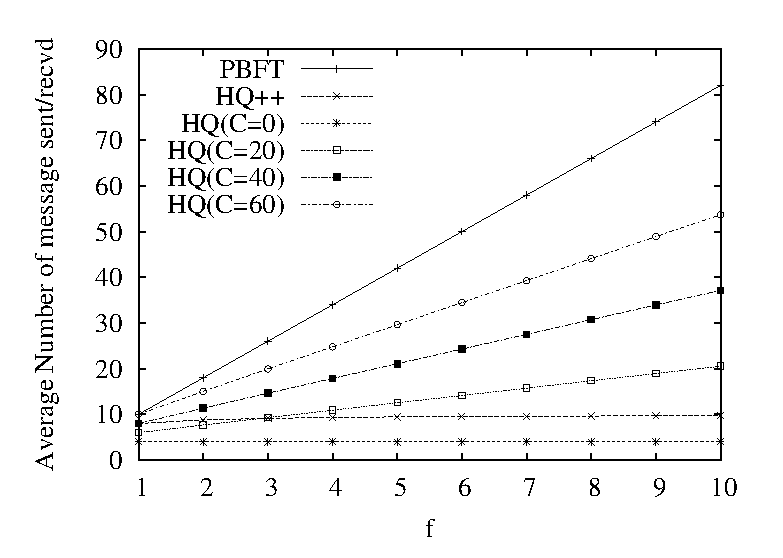
\includegraphics[width=3in]{Figures/Abs_Mesg_Count_Comp_PBFT_HQ.ps}
\caption{\textbf{[Preserialization]} Average message load on replicas per client
request. $C$ represents the probability of conflicting writes in the workload.
}
\label{fig:abs_mesg_count_comp} \end{figure}

\begin{figure}
\centering
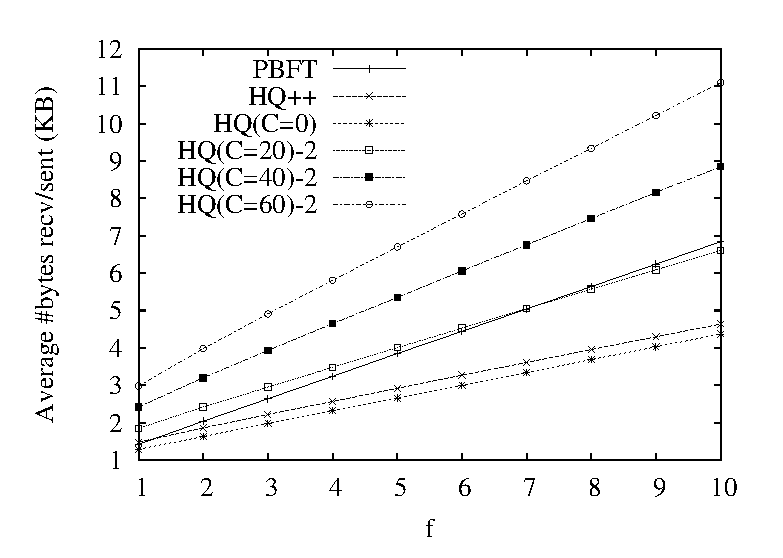
\includegraphics[width=3in]{Figures/Byte_Count_Comp.ps}
\caption{\textbf{[Preserialization]} Average number of bytes sent and received (in KB) at replicas
per client request. Under contention, we assume
that only 2 write requests conflict (overhead increases further if more requests conflict).
}
\label{fig:byte_count_comp}
\end{figure}

\begin{figure}
\centering
\includegraphics[width=3in]{Figures/Mesg_Count_Comp_BI_HQS.ps}
\caption{\textbf{[Relaxed consistency]} Average message load on the replicas
per client request.
}
\label{fig:mesg_comp_bi}
\end{figure}

\begin{figure}
\centering
\includegraphics[width=3in]{Figures/Byte_Count_Comp_BI_New.ps}
\caption{\textbf{[Relaxed consistency]} Average bytes (KB) sent/received by the replicas per client
request.
}
\label{fig:bytes_comp_bi_new}
\end{figure}

\fi

\if 0

\section{Related Work}

Say something about speculator~\cite{Speculator-sosp-05}.

Say something about relaxed consistency.

Say something about other, non-safe-hint optimizations of PBFT?

\fi



\section{Conclusion}
\label{sec:conclusion}
Speculative techniques are evident in many practical systems, e.g.,
branch prediction in compilers or speculation in distributed file
systems.  The safe hints pattern can be seen as an example of the
related ``trust but verify'' design philosophy. We allow replicas to let
an untrusted component of the system produce performance enhancing
hints.  These hints are verified before they can violate the
guarantees of the service implemented by the replication protocol.
Engineering issues involved in applying the pattern to BFT RSM involve
identifying effective hints that can be computed by individual
replicas yet can be safely verified, and recovering from a faulty hint
generator.

Nevertheless, even ignoring the (perhaps subjective) value of the safe
hint pattern, the contributions it has enabled us to construct stand on
their own.  By using serialization hints, HQ++ need never resolve conflicts, as long
as the hint generator is non-faulty. As an added benefit, HQ++
implements batching that traditional quorum protocols cannot
implement. Furthermore, BI-HQ opens up a new dimension in the BFT domain
by allowing applications to trade consistency for lower latency. We
foresee a broad range of further optimizations that thinking in terms of safe
hints may uncover. 



{
\footnotesize
\bibliographystyle{abbrv}
\bibliography{bft-scale}
}

\appendix
\section{BI-HQ++}

We now describe in detail how an additional safe hint improves the performance of
BI-HQ under fault free settings. Note that BI-HQ, as described in 
Section~\ref{sec:bihq}, requires $2f+1$ HQ protocol invocations to 
complete the synchronization round. With the pre-integration hint, we can reduce
the HQ invocations to just one. We now explain the modified synchronization round 
(all other aspects of BI-HQ remain unchanged).


\stitle{Pre-integration before synchronization}
Once a replica locally receives tentative requests of weight $\beta$ (a BI batch), it informs the hint
generating (UHG) replica of the HQ++ protocol and starts an associated timer. 
UHG replica then waits for $2f$ other replicas (including
its own) to submit their BI batches (each with weight less than $\beta$), and then
invokes the HQ protocol with a request formed by pre-integrating these BI batches.
Once HQ protocol linearizes the request, the SV module verifies the correctness of the pre-integration
hint. If correct, the requests contained
in the BI batches are executed in some deterministic order, marking completion of synchronization
round. If incorrect, UHG is changed and synchronization retried. If timer expires before
the synchronization round is complete, a replica submits its tentative batch to all other replicas,
causing them to invoke the synchronization round and a possible UHG change.

\stitle{Informal correctness} The safety property (i.e., consistency bounds are guaranteed) follows
directly from the arguement for the safety of BI-HQ protocol since replicas do not complete
the synchronization round unless they have seen $2f+1$ BI batches each with requests of weight less 
than $\beta$.  A faulty UHG may however affect the liveness
by not invoking the HQ protocol even after receiving a quorum of BI batches. This is not a problem
since the timers at the non-faulty replicas will expire, causing a UHG change.


\section{Preliminary Analysis}
We use three metrics to compare different protocols: (i) response latency,
(ii) average number of messages processed by the replicas per client request, and (iii) 
average number of bytes processed by the replicas per client request.
We configure both PBFT and HQ++ with batching size of 1. 


\stitle{Assumptions} We assume request and response payload of 256 bytes, TCP/IP header of 44 bytes,
8 byte MACs, 20 byte SHA-1 hash, 1 byte for client or replica ids, 4 bytes each for
the timestamps, sequence numbers and view identifiers.

\subsection{HQ++}
\stitle{Response latency}
HQ incurs 2 round trips or 4 message delays under normal case (i.e., no write contention and no
failurs). Contention resolution takes 4 additional message delays. 
HQ++ incurs 5 message delays similarly to PBFT under no failures.

\stitle{Message load} Under no write contention and faults, average number of messages processed
by replicas in HQ is 4. Contention resolution protocol takes additional messages. Clients submit 
write contention certificate to the replicas. A quorum of replicas send the $\msg{Start}$ message
to the primary replica. Primary initiate the PBFT protocol, which incurs $8f$ additional messages 
on every replica. So, contention resolution adds $10f$ messages on the primary while $8f+2$ on the
non-primary replicas. The number of messages, on an average, as processed by a replica 
is given by $4+f\delta(14+16f)/(2f+1)$, where $\delta$ is the fraction of write requests that
required contention resolution. We assume that the validation for the requests is performed during
the last phase of the PBFT protocol, this avoids additional messages and delay for the HQ protocol.

HQ++ incurs additional overhead on the hint generating replica compared to the HQ protocol: $2f$ messages
to be sent to the preferred quorum and receiving acknowledgements from the same quorum, a total
of $4+4f$ messages. Other replicas
receive 1 additional message from the hint generating replica and send an ACK to that replica compared 
to the HQ protocol, a total
of 6 message.
So, average message load of HQ++ is $4+(12f/(2f+1))$. PBFT incurs message
load of $(8f+2)$. 

Figure~\ref{fig:abs_mesg_count_comp} compares HQ, HQ++ and PBFT protocol according to the message
count. We observe two points: (i) HQ's message count approaches to that of PBFT as contention
increases, (ii) HQ++'s message count is significantly lower than that of PBFT and is slightly
higher than HQ with no write contention.



\stitle{Byte load}
Figure~\ref{fig:byte_count_comp} compares the
bytes processed per client request for PBFT, HQ and HQ++ protocol. We observe that
HQ++'s overhead is slightly higher than HQ's overhead with no write contention, which is expected due
to the pre-serialization. However, HQ++ incurs lower overhead than HQ under higher write contention.
HQ's overhead increases with write contention, surpassing the PBFT
protocol due to the additional work done by the HQ protocol before invoking the PBFT protocol and
the validation phase. HQ++ incurs less overhead than PBFT because it offloads part of the work to
clients. Also, both HQ++ and PBFT can implement batching, reducing the overheads further.

\begin{figure}[t]
\centering
\begin{minipage}[t]{0.47\textwidth}
\scalebox{0.6}{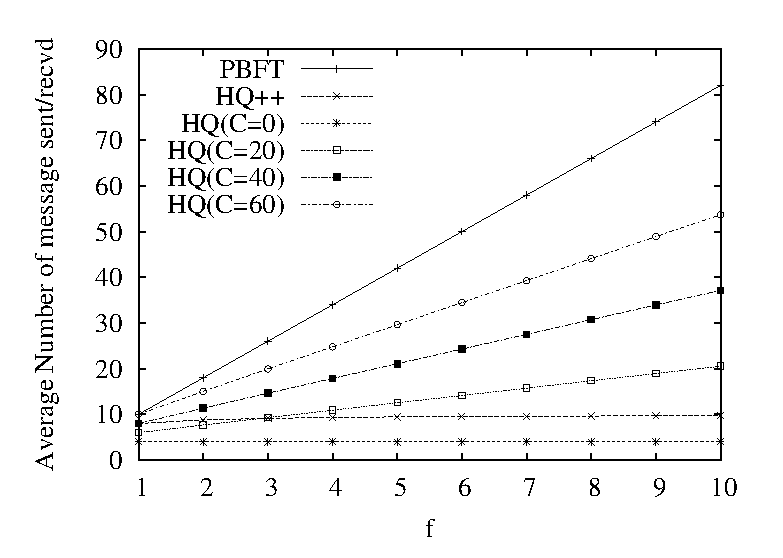
\includegraphics{Figures/Abs_Mesg_Count_Comp_PBFT_HQ.ps}}
\caption{\label{fig:abs_mesg_count_comp} [\textbf{Pre-serialization}] Average message load.
$C$ represents contention in the workload.}
\end{minipage}
\begin{minipage}[t]{0.47\textwidth}
\scalebox{0.6}{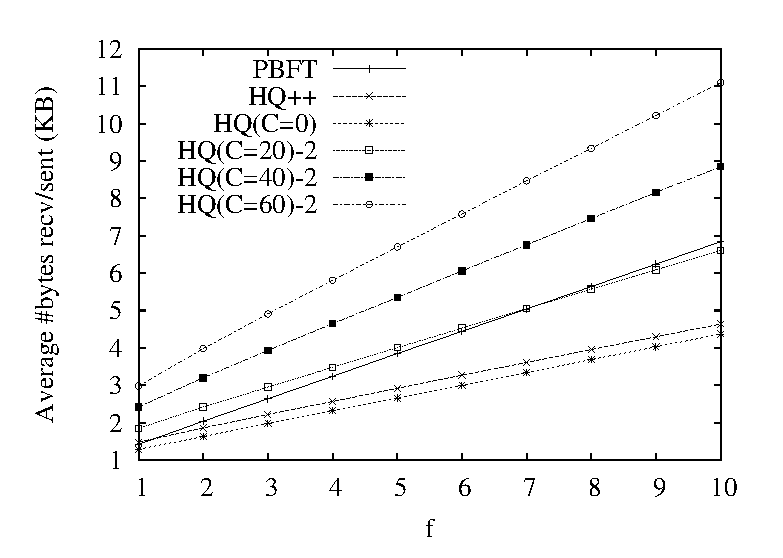
\includegraphics{Figures/Byte_Count_Comp.ps}}
\caption{\label{fig:byte_count_comp} [\textbf{Pre-serialization}] Average byte load.}
\end{minipage}
\end{figure}

\stitle{Summary} Our analysis shows that HQ is superior to both HQ++ and PBFT as long as there is
negligible write contention in the workload and both HQ++ and PBFT do not implement high
batching. With higher write contention, HQ++ is superior to both HQ and PBFT under fault free
settings and scales better with $f$.

\subsection{BI-HQ++}
Now, we consider the impact of relaxing the consistency requirements on the three metrics we
consider for comparision. We assume pre-integration of tentative updates before HQ is invoked
for linearization.

\stitle{Response latency} BI-HQ++ completes requests in 2 message delays that do not cause replicas
to initate the synchronization phase. Requests that trigger a synchronization round require
4 additional message rounds. With numerical error set to $\alpha$, the average request
latency is $2+(4/\beta)$ message delays.

\stitle{Message load} Again, requests that do not trigger a synchronization round incur 2 messages.
Synchronization round requires replicas to send their tentative updates to
the pre-integrator replica, which waits to collect a quorum of such tentative updates and then 
invokes the HQ protocol. Overall, pre-integrator replica
incurs $8f$ additional messages during synchronization round: $2f$ for receiving a quorum of 
tentative updates, $2f$ to send the first phase
request, $2f$ to receive the response to first phase and $2f$ to write back. Non pre-integrator
replicas incur additional 4 messages during synchronization round. 
So, the average load is $2+(16f)/((2f+1)\beta)$. 
Figure~\ref{fig:mesg_comp_bi} compares BI-HQ++ with HQ++ and PBFT with increasing numerical error.
We set $\alpha= x.(3f+1)$ and vary $x$. This ensures that as $f$ scales, $\beta$ remains fixed
for a given $\alpha$ ensuring that synchronization round is triggered at a rate of $\beta$ and 
independent of $f$. We observe that the message
load on replicas drops in proportion to the relaxation in consistency: higher the $\alpha$, lower
the message count.  


\stitle{Byte load} 
Figure~\ref{fig:bytes_comp_bi_new} compares the byte load at replicas. 
Again, we observe that as consistency is relaxed, the byte count overhead of BI-HQ++ 
drops proportionally. 

\begin{figure}[t]
\centering
\begin{minipage}[t]{0.47\textwidth}
\scalebox{0.6}{\includegraphics{Figures/Mesg_Count_Comp_BI_HQS.ps}}
\caption{\label{fig:mesg_comp_bi}[\textbf{Relaxed Consistency}] Average message load.}
\end{minipage}
\begin{minipage}[t]{0.47\textwidth}
\scalebox{0.6}{\includegraphics{Figures/Byte_Count_Comp_BI_New.ps}}
\caption{\label{fig:bytes_comp_bi_new}[\textbf{Relaxing Consistency}] Average byte load.}
\end{minipage}
\end{figure}

\stitle{Summary} One can view BI-HQ++ as HQ++ configured with 
batching. Higher the relaxation in consistency, higher the batch sizes and hence lower the overhead. 
However, one important distinction
is that BI-HQ++ does not sacrifice request latency whereas HQ++ configured with higher batching increases
the request latency since hint generator has to wait to collect a batch of requests before initiating
the request processing.

\if 0
\begin{table}
\centering
\begin{tabular}{|c|c|c|c|c|}
\hline
\small{Metrics}& \textit{\small{PBFT}} & \textit{\small{HQ}} & \textit{\small{HQ++}} & \textit{\small{BI-HQ++}}\\
\hline
\hline
\textbf{\small{Latency}} & 5/2 & 2+$\delta$.7/2 & 5/2 &  1+$\frac{2}{\beta}$ \\
\hline
\textbf{\small{Load-Non-Primary}} & $\frac{8f}{k}$+2 & 4+(2+8$f$)$\delta$ & 6 & 2+$\frac{4}{\beta}$ \\
\hline
\textbf{\small{Load-Primary}} & $\frac{8f}{k}$+2 & 4+10$f\delta$ & 4+4$f$ & 2+$\frac{8f}{\beta}$\\
\hline
\textbf{\small{Average load}} & $\frac{8f}{k}$+2 & 4+$\frac{(14+16f)f\delta}{(2f+1)}$ & 4+$\frac{8f}{(2f+1)}$ &  2+$\frac{16f}{((2f+1)\beta)}$ \\
\hline
\textbf{\small{Load-Client}}& 4$f$+2& 9$f$+4& 9$f$+4 & 4$f$+2\\
\hline
\end{tabular}
\caption{Comparing the performance of different protocols with respect to the latency and message load.
 $\delta$ represents the fraction of contending writes (affects only the HQ protocol). k is the batch size for the PBFT protocol. }
\label{tab:overhead_est}
\end{table}

\fi


\if 0

\section{Appendix}

\stitle{Limitations?} Say something about limitations, e.g., that you
can't get drop-dead optimal performance without violating structuring
constraints.

\stitle{Trick applicability} Pre-serialization works for all quorum
systems, as long as we can infer the identity of the current
hint generator from the committed application state.
Bounded-inconsistency without pre-integration works for all BFT
systems.  Bounded-inconsistency with a pre-integrator works for all BFT
systems where the identity of the pre-integrator can be based on
committed state.


\stitle{Patterns and Reality} As with any system structuring pattern
(e.g., layering or the end-to-end principle), the safe hint pattern is
the launch pad, not the destination of a protocol designer's task.
Often further efficiencies can be obtained by violating the strict
boundaries of the pattern, typically at a great potential maintenance or
engineering cost.  In the case of BFT services, this boundary violation
also carries with it the need for extra validation effort, since now the
designers must prove the correctness properties for their entire design,
not just for the new components bracketing the original BFT system.  For
instance, the version of HQ++ discussed in Section~\ref{sec:hq++} could
be made more efficient in terms of messages sent and message delays
required by combining the UHM with one of the replicas and leaving the
HQ client-replica protocol otherwise untouched.  Though this would not
change the reason for which HQ++ performs better under contention, it
might further improve its overhead.  It would also, however, require a
rigorous proof that the modification to HQ does not invalidate its
guarantees.


\stitle{Further applicability} Other instances of safe hints.

Bells and whistles to the serializer (failure detector for
serializer)

Reducing load on serializer

Applications for \bihq

Systems such as Q/U, PBFT, and HQ are optimal for different areas
in the parameter space. For instance, for small replica sets, Q/U is
more efficient than HQ at low concurrency and PBFT is more efficient
than either at high concurrency. A fully adaptive systems would ideally
pick and choose which of Q/U, HQ, or PBFT (or their descendants and
competitors) to use according to a running estimate of the offered
workload. An untrusted protocol selector could perform that task. The
replica quorum executing the request stream arriving from the underlying
replicated state machine protocol could then validate the safety of the
request, as well as perhaps the safety of the choice of protocol based
on provable observations (e.g., a certificate of high recent concurrency
made of k concurrency certificates with timestamps within T values).

Undo during conflict resolution

Read requests.

hint generators for different objects (use h(view number, sequence
number, object ID) instead of h(view number, sequence number)).

hint generators chosen from the clients, not from the replicas?

Transactions.

Slow hint generators.


\begin{figure}
\centering
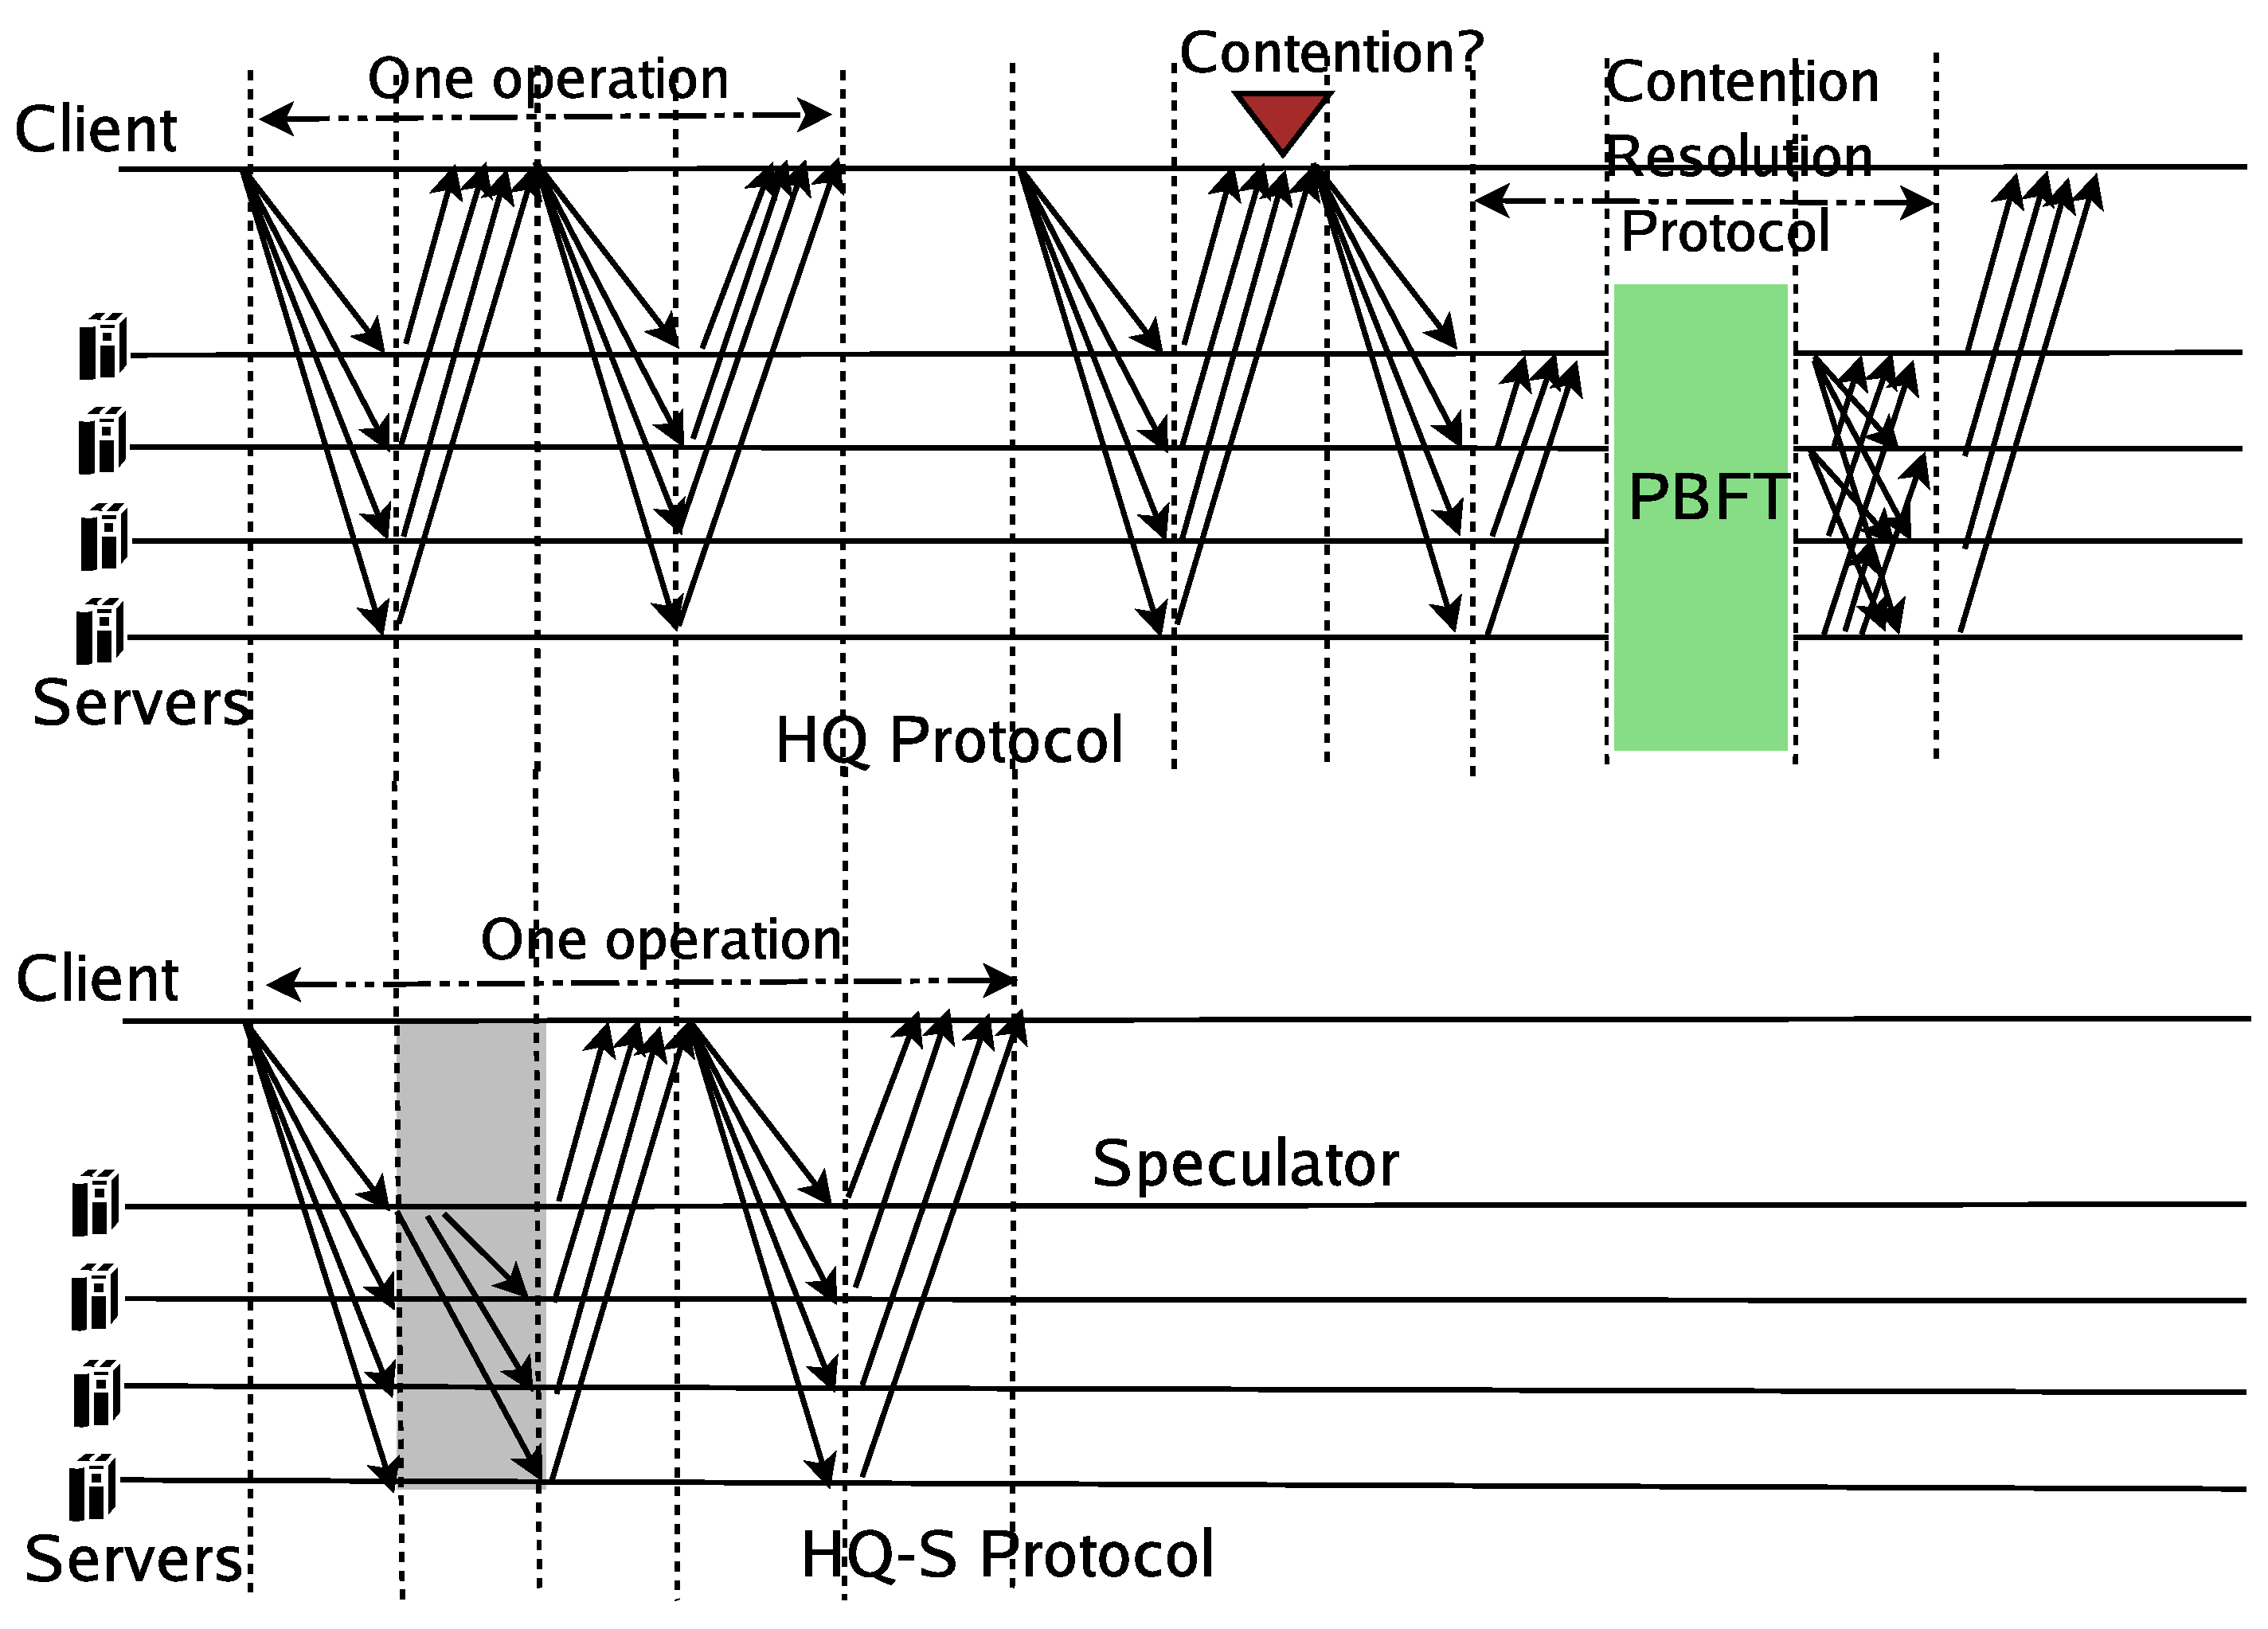
\includegraphics[width=3.2in]{hq++.eps}
\caption{Incorporating the hint generator in the HQ protocol. Note that HQ++
takes 5 message delays and HQ takes 4 message delays.  The extra delay is
due to the hint generator.}
\label{fig:hq++}
\end{figure}

Assumptions

Proof is provided in a separate technical report~\cite{}.

Many optimizations exist (e.g., second round of retransmission before
hint generator change, as with PBFT).



We are really great!


\fi





\if 0
\section{Target Applications}
\label{sec:applications}

\stitle{Key characteristics} Should be able to tolerated relaxed consistency.
Multiple writer. 

\stitle{Application that can tolerate weak consistency}
Here we identify the set of target applications that can benefit from the \bihq
protocol. So far we have:
\begin{itemize}
\item{} Domain Name System (DNS)
\item{} Checking invariants in distributed systems, such as content distribution networks (CDN's).
\item{} Routing Control Platform [NSDI'05]. 
\end{itemize}

\stitle{DNS} DNSSEC provides authentication to DNS but not widely used. DNS typically does not experience lot
of update/write workload. Majority of operations are queries. Some BFT based solutions have been proposed 
(from Liskov's group, not published) that tolerate faults in the nameservers. All nameservers are replicated to 
$3f+1$ replicas. The biggest problem with legacy DNS is the load on the nameservers higher up in the hierarchy.
Legacy DNS allows caching of DNS records and uses TTL for cache coherency. However, setting the right TTL is a burden
and introduces a tradeoff between overhead and coherency. This is true even for the BFT based DNS. There are some
proposals for a new DNS architecture (CoDoNS) which attempt to solve this problem via using an overlay to disseminate
updates in a timely fashion. \note{Need to think more on this one.}


\stitle{CDN} Publishers control membership, however need a mechanism to enforce certain invariants, e.g., 
each non-leaf member has taken at least a given number of children (control plane verification) and 
has forwarded sufficient number of data packets (data plane verification). \note{Again, need to think on this one.}

\stitle{RCP} RCP is a new proposal to deal with the complexity of identifying the optimal BGP paths for each 
router in an AS and to avoid the usual problems of routing loops being formed when distributed protocols are used, i.e., when
each router independently calcuates routes for itself. 
RCP obtains the full connectivity of the AS and the external BGP connectivity information to calculate such routes. However, a single 
RCP is problematic (single point of failure). Multiple RCP's needed to tolerate failure. However, what happens if some RCP's are faulty? 
(Consider for now that the routers are fault-free in the AS). Traditional BFT protocols can be used but there are opportunities to relax
the consistency requirements. First, routing protocols give best effort guarantee, so using a strict consistency BFT protocol
is probably an overkill. Moreover, since RCP is responsible for calculating the paths for every router in an AS, doing a BFT per
update and re-calculating the path for every router after such update is probably going to be too expensive. 
In fact, some router vendors do not reflect updates (of lower significance) immediately. 
They do it periodically. However the updates which affect the connectivity to tunnel endpoints are immediately reflected. 
This suggests that assigning different weights to different kind of updates can be used to identify when to do the BFT commit. 

\stitle{\bihq for RCP} Ideal state that RCP should achieve: each router's path is calculated instantly as soon as 
an update appears in the system. This is the ideal or 
strict consistency. Our goal is to relax this consistency. One idea: conit of each update is either the change in the link
weights (for link weight change updates) or some higher value if the link goes down. Numerical error is simply the weight of
such updates. This is fine, however its impact on usefulness of RCP is not clear. For example, can we answer a question like
this: at any time, what fraction of routes computed by RCP are optimal? What is its relationship with numerical error?
\fi

\end{document}


